\documentclass[12pt]{article}
\usepackage{hyperref}
\usepackage{graphicx}
\usepackage[table,xcdraw]{xcolor}
\usepackage{listings}
\usepackage{float}
\usepackage{fixltx2e}
\restylefloat{table}
\graphicspath{ {images/} }

\sloppy
\definecolor{lightgray}{gray}{0.5}
\setlength{\parindent}{0pt}

\definecolor{darkgreen}{rgb}{0,0.6,0}
\definecolor{ident}{rgb}{.3,.0,.2}


\lstset{language=matlab}
\lstset{showstringspaces=false}
\lstset{frame=L}
\lstset{breaklines=true}
\lstset{basicstyle=\footnotesize\ttfamily\bfseries}
\lstset{commentstyle=\color{darkgreen}}
\lstset{keywordstyle=\bfseries\color{blue}}
\lstset{numberstyle=\color{black}}
\lstset{rulecolor=\color{black}}
\lstset{numbers=left}
\renewcommand{\thefootnote}{\fnsymbol{footnote}}

\title{Quadcopter Design and Build Log}
\author{M Dobosz}

\begin{document}
\begin{titlepage}
\vspace*{-4.5cm}
\hspace*{-4.1cm}
{\let\newpage\relax\maketitle}

\begin{table}[b]
\begin{center}
\begin{tabular}{| l | l | l |}
\hline
\textbf{Revision Date} & \textbf{Description} \\ \hline
01/09/18 & Initial document \\ \hline
02/11/18 & Update to use mavic frame design \\ \hline
03/31/18 & Added electronics section \\ \hline
05/25/18 & Updated electronics section and added final BOM
\end{tabular}
\end{center}
\end{table}
\end{titlepage}


\pagebreak
\tableofcontents
\pagebreak

\section{Introduction}

The purpose of this document is to record and explain the design process of a quadcopter and why each decision was made. Since I have little experience with the design process, all steps performed for this project were made up as I went along and may or may not be representative of the real-world design process. This document was created to better organize my thoughts and each decision I made for future collaborators to get up to speed and to learn what is going on. All information that is obtained from outside sources is referenced with footnotes, however only the url or website is noted and no proper citation format is used. All information is presented in a way that someone with little to no technical experience can understand (hopefully).
\\

A quadcopter is a four rotor manned or unmanned vehicle used mostly for aerial photography. Many sensors such as gyroscopes and accelerometers, which are located on the flight controller, are used to provide the aircraft with feedback on altitude, acceleration, orientation, etc. The "heart" of the quadcopter is the flight controller, which takes data from its sensors and the receiver and sends the information to the ESCs\footnote{Electronic Speed Controller; used to convert the DC voltage from the flight controller to a three-phase AC signal for the motors} More info can be found \href{https://en.wikipedia.org/wiki/Quadcopter}{\color{cyan}here}.
\\

\section{Objectives}

The main objectives of the project are:
\renewcommand{\labelitemi}{\textperiodcentered}
\begin{itemize}
\item a minimum of 10 minutes of flight time
\item easily replaceable parts in the event of a failure or crash
\item small enough to carry in a backpack
\item easily understandable design so people with minimal technical experience can learn
\item price under \$350 CAD (not including radio, tools and taxes/duty)
\end{itemize}

All decisions that must be made for which materials to use, physical design, etc. will follow these rules strictly.
\\

Secondary objectives include:
\renewcommand{\labelitemi}{\textperiodcentered}
\begin{itemize}
\item GPS support
\item sonar for low-altitude hold
\item space and bracket(s) for mounting of a GoPro camera in the future for aerial photography
\item use of Hologram's Nova cellular modem for communication, GPS, or data logging
\end{itemize}

Two main design sections will be considered, the frame and the electronics. The frame will consist of the structural components of the quadcopter where all the electronic components will be mounted. The electronic components will include the flight controller, motors, ESCs, battery and receiver. 
\\

The main restriction imposed on this project is cost. Most, if not all, decisions are made with cost as one of the heaviest factors. Time and difficulty are not as important as this project does not have a deadline and new skills can be learned along the way.
\\

For all custom components, either SolidWorks or Altium Designer will be used, if needed.

\section{Frame Design}
\begin{figure}[H]
\caption{Mavic Pro Clone}
\centering
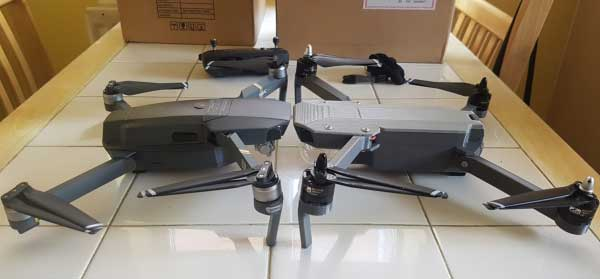
\includegraphics[scale=0.6]{mavic.png}
\end{figure}

The frame design is the section that will cause the most trouble, as I have little to no mechanical experience and designing a frame that is both lightweight and durable is an entire project in itself. To simplify the designing of the frame, CdRsKuLL's Mavic F3 v4.1 frame from Thingiverse will be used. \href{http://diyrc.co.uk/3d-printed-mavic-clone/mavic-clone-stl-files-version-3-0-f3/}{\color{cyan}Full details can be found here.}

\subsection{Frame Material}

According to Simplify3D, the estimated volume of the frame when 3D printed will be 250 cm\textsuperscript{3}. Depending on the material chosen, a weight can be calculated and suitable motors can be selected.
\\

Five materials were considered for the frame design: PLA (Polylactic Acid), ABS (Acrylonitrile Butadiene Styrene), Carbon Fiber PLA and Nylon and PETG (Polyethylene Terephthalate Glycol). The advantages and disadvantages of each material were investigated and are presented below.
\\

\vspace{5mm}
\textbf{PLA:}
\renewcommand{\labelitemi}{\textperiodcentered}
\begin{itemize}
\item[+] easy to print with
\item[+] biodegradable
\item[-] warps if exposed to sunlight for too long
\item[-] lower structural stability compared to other materials
\item[Price:] \$31 CAD per kg 
\item[Density:] 1.25g/cm\textsuperscript{3}
\end{itemize}
\vspace{5mm}


\textbf{ABS:}
\renewcommand{\labelitemi}{\textperiodcentered}
\begin{itemize}
\item[+] high durability
\item[+] flexible and lightweight
\item[-] unpleasant fumes released when printing
\item[-] prone to warping without heated enclosure
\item[Price:] \$30 CAD per kg
\item[Density:] 1.05g/cm\textsuperscript{3}
\end{itemize}
\vspace{5mm}

\textbf{CF PLA:}
\renewcommand{\labelitemi}{\textperiodcentered}
\begin{itemize}
\item[+] very high durability mimicking carbon fiber
\item[+] prints like PLA
\item[-] required hardened nozzle
\item[-] expensive
\item[Price:] \$60 CAD per kg + nozzle
\item[Density:] 1.30g/cm\textsuperscript{3}
\end{itemize}
\vspace{5mm}

\textbf{Nylon:}
\renewcommand{\labelitemi}{\textperiodcentered}
\begin{itemize}
\item[+] strong. durable and flexible
\item[+] less brittle than PLA and ABS
\item[-] high temperature required for printing
\item[-] emits toxic fumes when printing
\item[Price:] \$50 CAD per kg
\item[Density:] 1.15g/cm\textsuperscript{3}
\end{itemize}
\vspace{5mm}

\textbf{PETG:}
\renewcommand{\labelitemi}{\textperiodcentered}
\begin{itemize}
\item[+] high durability and flexibility
\item[+] does not shrink
\item[+] does not warp
\item[-] requires fine tuning of printer settings
\item[Price:] \$40 CAD per kg
\item[Density:] 1.27g/cm\textsuperscript{3}
\end{itemize}

After extensive consideration it was decided that PETG would be used. PETG combines the simplicity of PLA printing with the strength of ABS. The relatively low price compared to carbon fiber also makes it the superior choice. The only downside that may arise is that PETG is the heaviest material out of the three (PLA, ABS, PETG), but shouldn't cause too much of an issue. 
\\

To calculate the total weight of the frame, the simple equation below was used:

\begin{equation}
density \cdot volume = 1.27\ g/cm\textsuperscript{3} \cdot 250\ cm\textsuperscript{3} = {\color{red}317.5\ g}
\end{equation}

The battery and electronics weight will be considered in a later section.

\subsection{Frame Finishing}
3D printing produces a rough looking frame with a stepping effect due to the layer transitions. Although this does not affect the functionality of the aircraft, aesthetics will be considered. A simple combination of body filler (i.e. Bondo car body filler), sanding and spray paint should be sufficient. (\href{https://www.youtube.com/watch?v=NR2RF40Oq6M}{\color{cyan}This video will be followed.})

\section{Electronics}

\subsection{Motors and Propellers}
The recommended motor that the author used is the Black Widow 2208 1200KV, however this motor is discontinued and no longer available off of HobbyKing.
\\

The motors that will be used are the EMAX MT2213-935KV motors. Using an 8 inch propeller, 6 - 7.1 amps are used to give 440 - 500 g of thrust. This is enough to lift the quadcopter and allow it to perform stunts.
\\

\begin{figure}[!htb]
\caption{Motor Specs}
\centering
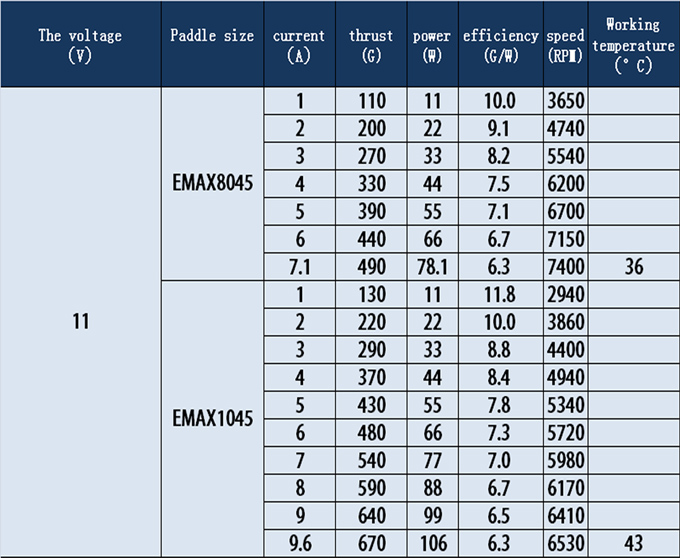
\includegraphics[scale=0.4]{motor_specs.jpg}
\end{figure}

The motors will be arranged in the Quad-x configuration shown below:

\begin{figure}[!htb]
\caption{Motor orientation for Quad-X mode}
\centering
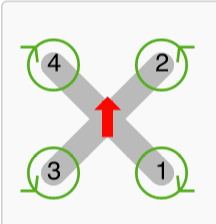
\includegraphics[scale=0.5]{quadx.png}
\end{figure}


\subsection{ESCs}
The ESCs that will be used are the Racerstar 20A opto ESCs. They provide enough current for the motors and are very small in size.

\subsection{Battery}
The recommended battery is the Multistar 3000mAh 3S Li-Po. This battery will be used as it is affordable and has a high capacity. The battery is 188g with dimensions 107 x 36 x 28mm. 
\\

The battery is rated for 10C, meaning that it can provide a continuous current of 30A. It is rated for 20C burst current, meaning it can provide a current of 60A for 10 seconds. The quadcopter is rated to draw around 30A maximum, so this battery is more than enough.
\\

Assuming ideal conditions, the flight time can be calculated using the following formula:
\\

\begin{equation} 
\frac{battery\ capacity}{load\ current} = \frac{3,000\ mAh}{16,393.4\ mA} = .183\ hours = 10.98\ minutes
\end{equation}
This time meets the required minimum 10 minute flight time.

\subsection{Flight Controller and Receiver}
The recommended flight controller is the \href{https://www.banggood.com/Upgrade-NAZE32-F3-Flight-Controller-Acro-6-DOF-Deluxe-10-DOF-for-Multirotor-Racing-p-1010232.html?ID=17&cur_warehouse=CN}{\color{cyan}SP Racing F3 Deluxe.} The one mentioned in the guide is the older version which uses a serial to USB adapter instead of straight USB. It also lacks some of the newer features such as i\textsuperscript{2}c\footnote{Inter-Integrated Circuit; pronounced I-squared-C. A communication protocol that allows peripherals to be controlled by a master circuit, in this case an OLED screen will be driven by the flight controller} which can be used for an OLED\footnote{Organic Light Emitting Diode; a type of display that has a high contrast ratio, used often for small electronics for its low power consumption and price.} screen. For this project, the newer version will be used for its updated features and availability.
\\

This flight controller features an accelerometer, gyroscope, barometer and magnetometer (compass). Optionally, a GPS and sonar can be added (which in the case of this quadcopter, will be added). An RGB LED and buzzer can also be added to show the status of the flight controller. There are many other advanced features that are beyond the scope of this project, and therefore will be ignored.
\\

The receiver that will be used will be the \href{https://hobbyking.com/en_us/frsky-x4rsb-3-16ch-2-4ghz-accst-receiver-w-telemetry.html}{\color{cyan}FrSky X4RSB} for its SBUS\footnote{Radio control communication protocol.} capability and high build quality. 

\subsection{Miscellaneous Electronics}
The final electronics will be the sensors such as the \href{https://www.banggood.com/NZ-GPS-For-NAZE32-Flip32-6dof-10dof-Best-For-QAV250-ZMR250-Multicopter-Quadcopter-p-1015134.html}{\color{cyan}GPS}, sonar, LED, buzzer, etc. These all interface with the flight controller and provide it with any environmental data it may need. For example, the GPS can be used for flight logging, return to home, and pre-planned routes. The sonar is used to allow for low-altitude hold. 

\section{Software}
The quadcopter will be programmed with iNav, a fork of CleanFlight.

\section{Bill of Materials}
\begin{figure}[h]
\caption{BOM}
\centering
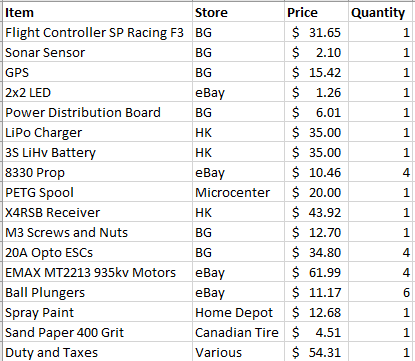
\includegraphics{bom.png}
\end{figure}

The total cost is \$392.98 CAD. This is within the \$350 CAD budget as the duties, taxes and tools bring it over.

\section{Appendix}

\end{document}
